\documentclass[border=10pt]{standalone}
\usepackage[svgnames]{xcolor}
\usepackage{amsmath}
\usepackage{pgfplots}
\pgfplotsset{compat=newest}
\usepackage[sfdefault]{FiraSans}
\usepackage{FiraMono}
\renewcommand*\familydefault{\sfdefault}
\begin{document}
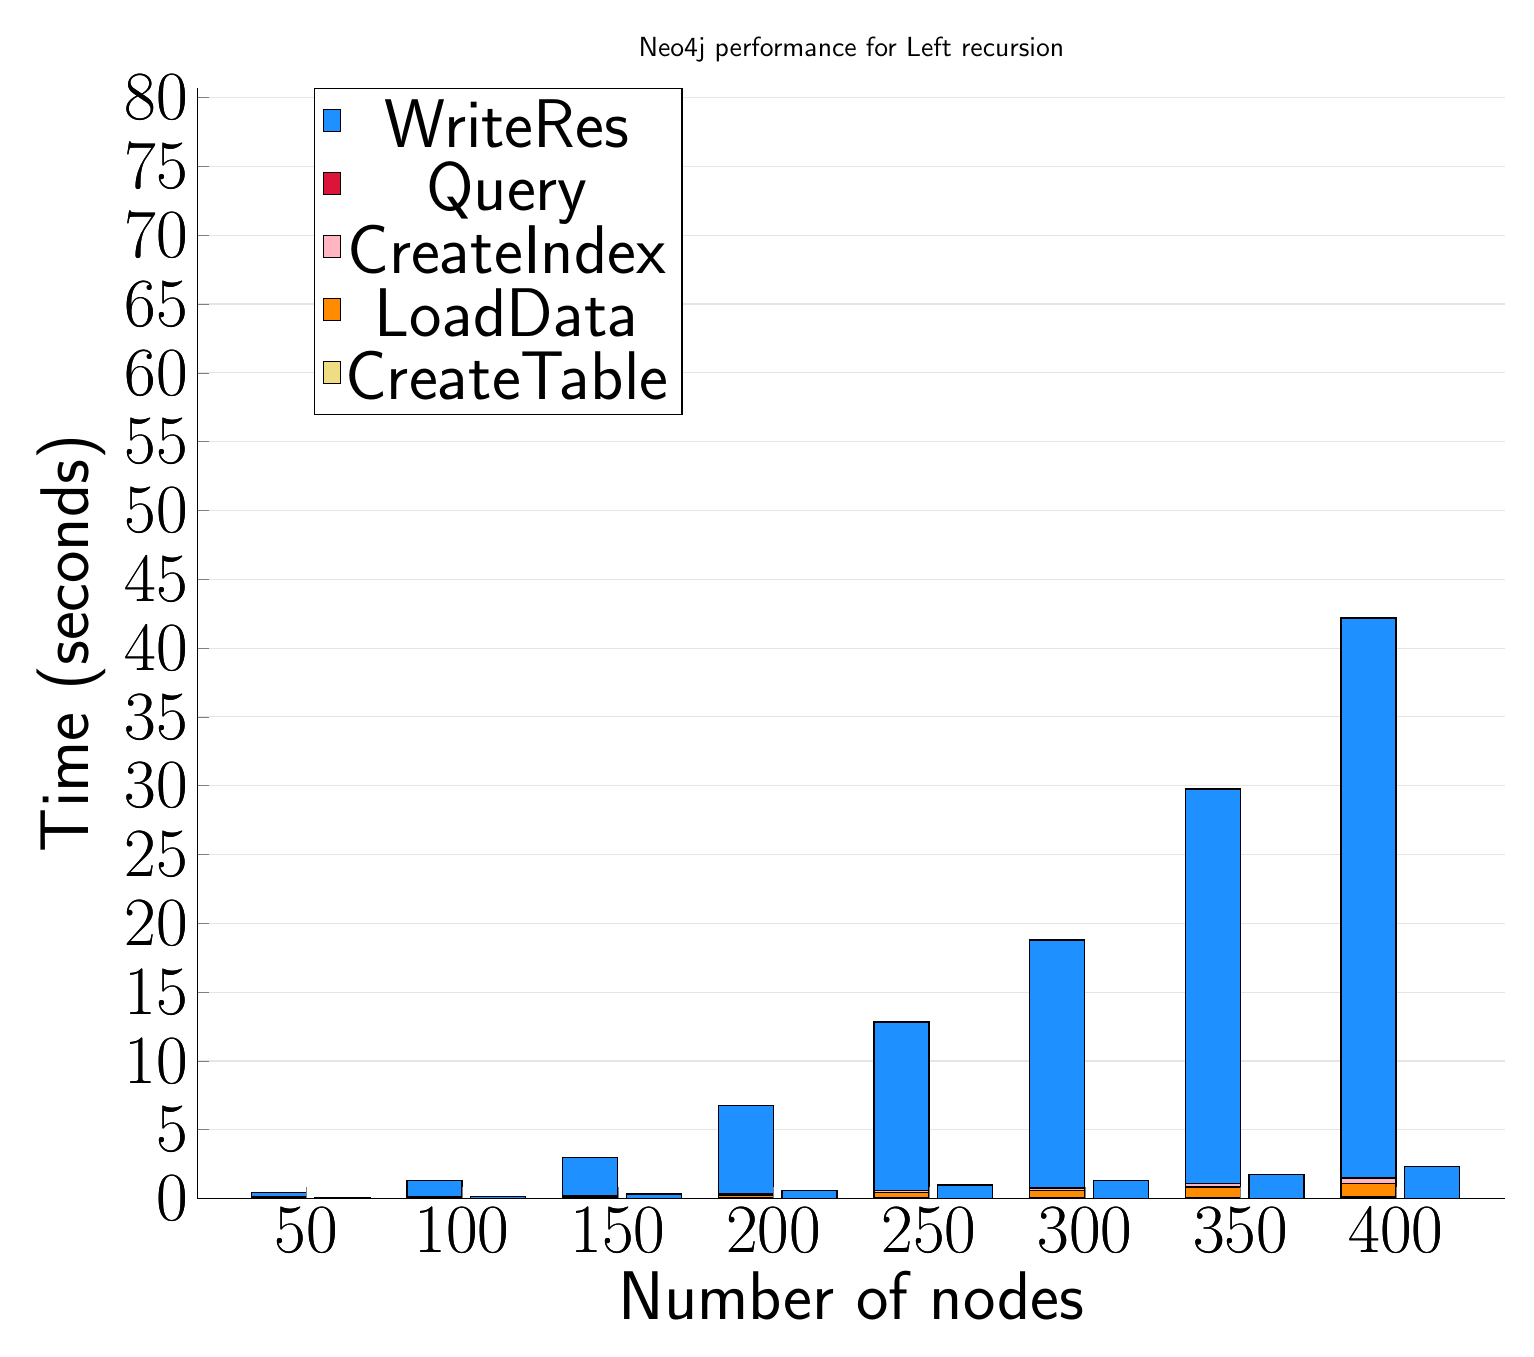
\begin{tikzpicture}
\begin{axis}[
   ybar stacked,
   title={Neo4j performance for Left recursion},
   bar shift=-10pt,
   width=1.5\textwidth,
   bar width=0.7cm,
   ymajorgrids, tick align=inside,
   major grid style={draw=gray!20},
   xtick=data,
   ymin=0, ymax=80.70666666577259,
   axis x line*=bottom,
   axis y line*=left,
   enlarge x limits=0.1,
   legend style={
       at={(0.23, 1)},
       anchor=north,
       legend columns=1,
       font=\Huge,
   },
   ylabel={Time (seconds)},
   xlabel={Number of nodes},
   label style={font=\Huge},
   tick label style={font=\Huge},
]
\addlegendimage{fill=DodgerBlue, draw=black, line width=0.2pt}
\addlegendentry{WriteRes}
\addlegendimage{fill=Crimson, draw=black, line width=0.2pt}
\addlegendentry{Query}
\addlegendimage{fill=LightPink, draw=black, line width=0.2pt}
\addlegendentry{CreateIndex}
\addlegendimage{fill=DarkOrange, draw=black, line width=0.2pt}
\addlegendentry{LoadData}
\addlegendimage{fill=LightGoldenrod, draw=black, line width=0.2pt}
\addlegendentry{CreateTable}
\addplot +[fill=LightGoldenrod, draw=black, line width=0.5pt] coordinates {
    (50, 0.013333335518836975)
    (100, 0.013333330551783243)
    (150, 0.02666666607062022)
    (200, 0.033333333830038704)
    (250, 0.05999999741713206)
    (300, 0.05666666726271311)
    (350, 0.08666666597127914)
    (400, 0.10999999940395355)
};
\addplot +[fill=DarkOrange, draw=black, line width=0.5pt] coordinates {
    (50, 0.04333333422740301)
    (100, 0.0533333346247673)
    (150, 0.09999999900658925)
    (200, 0.21666666368643442)
    (250, 0.3933333332339923)
    (300, 0.5333333313465118)
    (350, 0.7600000003973643)
    (400, 0.9833333318432173)
};
\addplot +[fill=LightPink, draw=black, line width=0.5pt] coordinates {
    (50, 0.023333333432674408)
    (100, 0.02999999870856603)
    (150, 0.04333333422740301)
    (200, 0.10666666676600775)
    (250, 0.1399999981125196)
    (300, 0.17333333442608514)
    (350, 0.2433333322405815)
    (400, 0.3466666688521703)
};
\addplot +[fill=Crimson, draw=black, line width=0.5pt] coordinates {
    (50, 0.02333333094914754)
    (100, 0.023333335916201275)
    (150, 0.0066666677594184875)
    (200, 0.023333333432674408)
    (250, 0.0)
    (300, 0.006666665275891622)
    (350, 0.010000000397364298)
    (400, 0.049999999503294625)
};
\addplot +[fill=DodgerBlue, draw=black, line width=0.5pt] coordinates {
    (50, 0.34666666636864346)
    (100, 1.2000000004967053)
    (150, 2.826666665573915)
    (200, 6.383333335320155)
    (250, 12.22999999920527)
    (300, 18.030000001192093)
    (350, 28.656666666269302)
    (400, 40.706666665772595)
};
\end{axis}
\begin{axis}[
   ybar stacked,
   bar shift=13pt,
   width=1.5\textwidth,
   bar width=0.7cm,
   ymajorgrids, tick align=inside,
   major grid style={draw=none},
   xtick=data,
   ymin=0, ymax=80.70666666577259,
   axis x line*=none,
   axis y line*=none,
   enlarge x limits=0.1,
   label style={font=\Huge},
   tick label style={font=\Huge},
]
\addplot +[fill=LightGoldenrod, draw=black, line width=0.5pt] coordinates {
    (50, 0.003333333333333336)
    (100, 0.009999999999999986)
    (150, 0.0066666666666666706)
    (200, 0.0)
    (250, 0.00999999999999997)
    (300, 0.0066666666666666515)
    (350, 0.003333333333333336)
    (400, 0.006666666666666668)
};
\addplot +[fill=DarkOrange, draw=black, line width=0.5pt] coordinates {
    (50, 0.0)
    (100, 0.003333333333333336)
    (150, 0.0)
    (200, 0.0)
    (250, 0.0)
    (300, 0.0)
    (350, 0.0)
    (400, 0.0)
};
\addplot +[fill=LightPink, draw=black, line width=0.5pt] coordinates {
    (50, 0.0)
    (100, 0.0)
    (150, 0.0)
    (200, 0.0033333333333333344)
    (250, 0.0)
    (300, 0.0033333333333333375)
    (350, 0.0033333333333333322)
    (400, 0.006666666666666673)
};
\addplot +[fill=Crimson, draw=black, line width=0.5pt] coordinates {
    (50, 0.0033333333333333344)
    (100, 0.0)
    (150, 0.003333333333333336)
    (200, 0.0)
    (250, 0.0)
    (300, 0.0)
    (350, 0.0)
    (400, 0.0)
};
\addplot +[fill=DodgerBlue, draw=black, line width=0.5pt] coordinates {
    (50, 0.04)
    (100, 0.1366666666666667)
    (150, 0.32)
    (200, 0.5966666666666667)
    (250, 0.9666666666666668)
    (300, 1.3066666666666669)
    (350, 1.7599999999999998)
    (400, 2.3333333333333335)
};
\end{axis}
\end{tikzpicture}

\end{document}
